\chapter{Основная часть}
\section{Имеющиеся данные}
В рамках программы SAHR были записаны ЭКГ (использовалось только первое отведение) 1800 москвичей преклонного возраста (55--91 год). Из них 46\% мужчин. 81\% из них чувствовал себя во время обследования хорошо, 19\% -- плохо. 49\% имеют высшее образование. Также имеются данные об общем состоянии физического и психического здоровья каждого человека, индекс массы тела и множество других данных о его состоянии (заболевание, курит ли человек, с какого возраста и т.п.) Запись каждого ЭКГ производилась с помощью холтеров в течение суток. В это же время за человеком велось дополнительное наблюдение и было известно, в какой промежуток времени он спал, а в какой -- бодрствовал.
\section{Постановка задачи}

Цели работы: анализируя данные ЭКГ, определить, в какие промежутки времени человек спал, а в какие -- бодрствовал, исследовать возможность предсказания болезней и самочувствия человека. 
Для решения данных задач были проведены работы по выделению признаков и исследования их информативности.

\section{Актуальность задачи}
Электрокардиография -- самый распространенный клинический инструмент, который измеряет электрическую деятельность сердца с поверхности тела. Сигнал ЭКГ, или проще вариабельности сердечного ритма содержит много интересной информации о человеке. Сейчас медицинские институты в дополнение к существующим базам данных (SAHR, AHA DB, ESC DB и т. д.) формируют новые. Также разработано множество новых технологий и приборов, таких как фитнесс-браслеты, специальные чехлы для телефонов, мониторы-холтеры и др., позволяющие человеку без каких либо трудностей и специального медицинского оборудования круглосуточно (или в любое удобное для него время) записывать информацию о своем пульсе и отправлять эти данные  для анализа в медицинские центры. У врачей появилась возможность постоянно контролировать состояние пациента. Популярность подобных носимых устройств для мониторинга здоровья растет с каждым годом. Они позволяют человеку быть подвижным, заниматься своими делами и в это же время собирать данные о своем здоровье в "естественной" среде. Точность этих приборов уступает специализированным установкам -- но даже по их сигналу можно многое сказать о человеке. 

Качество и длительность сна имеют важное значение для медицинской диагностики. Но на практике сложность процедуры классической полисомнографии накладывает существенные ограничения для ее применения. Несмотря на множество информации, которую предоставляют носимые электронные устройства и исследований в этом направлении, на сегодняшний день нет хороших научных доказательств, представленных публике, о том, что они могут оценить продолжительность сна с высокой точностью.

\section{Обработка ЭКГ сигнала и выделение RR-пиков}
\subsection{Выделение RR-сигнала}

Вначале нам необходимо найти местоположение R-пиков. Для этого данный сигнал обрабатывался рядом фильтров. При этом не имеет значения, какой вид примет QRS-комплекс. Фильтрация производится на основе дискретного преобразования Фурье (ДПФ): проводится ДПФ, зануляются нужные коэффициенты и производится обратное преобразование ДПФ. Зануление нужных коэффициентов реализуется с помощью ФНЧ и ФВЧ. Границы фильтров подбирались индивидуально для каждого человека, в зависимости от распределения частот после преобразования Фурье.

Вид сигнала после применения фильтров можно наблюдать на рис.  \ref{ris:filter_ekg}

\begin{figure}[h]
	\begin{minipage}[h]{0.47\linewidth}
		\center{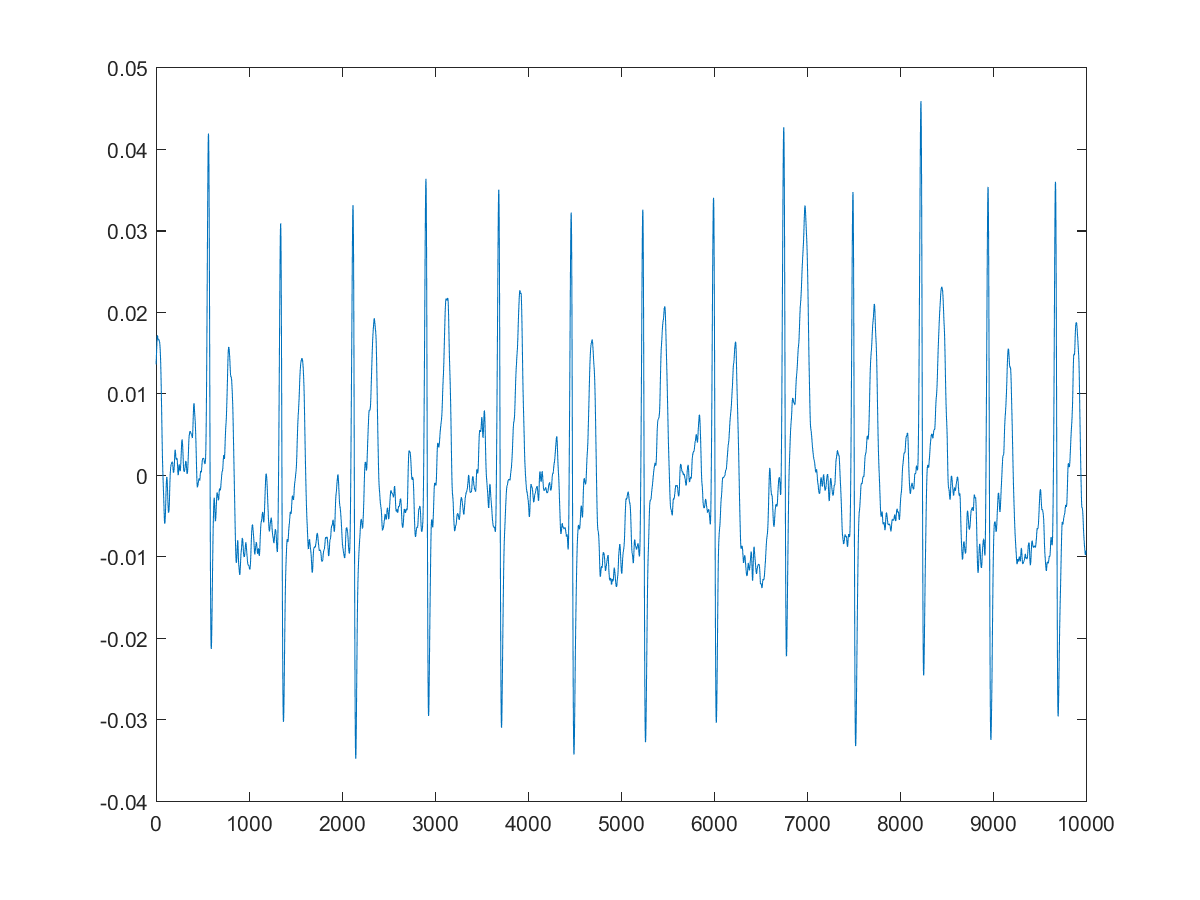
\includegraphics[width=1\linewidth]{filtered_ekg_base}} a) \\
	\end{minipage}
	\hfill
	\begin{minipage}[h]{0.47\linewidth}
		\center{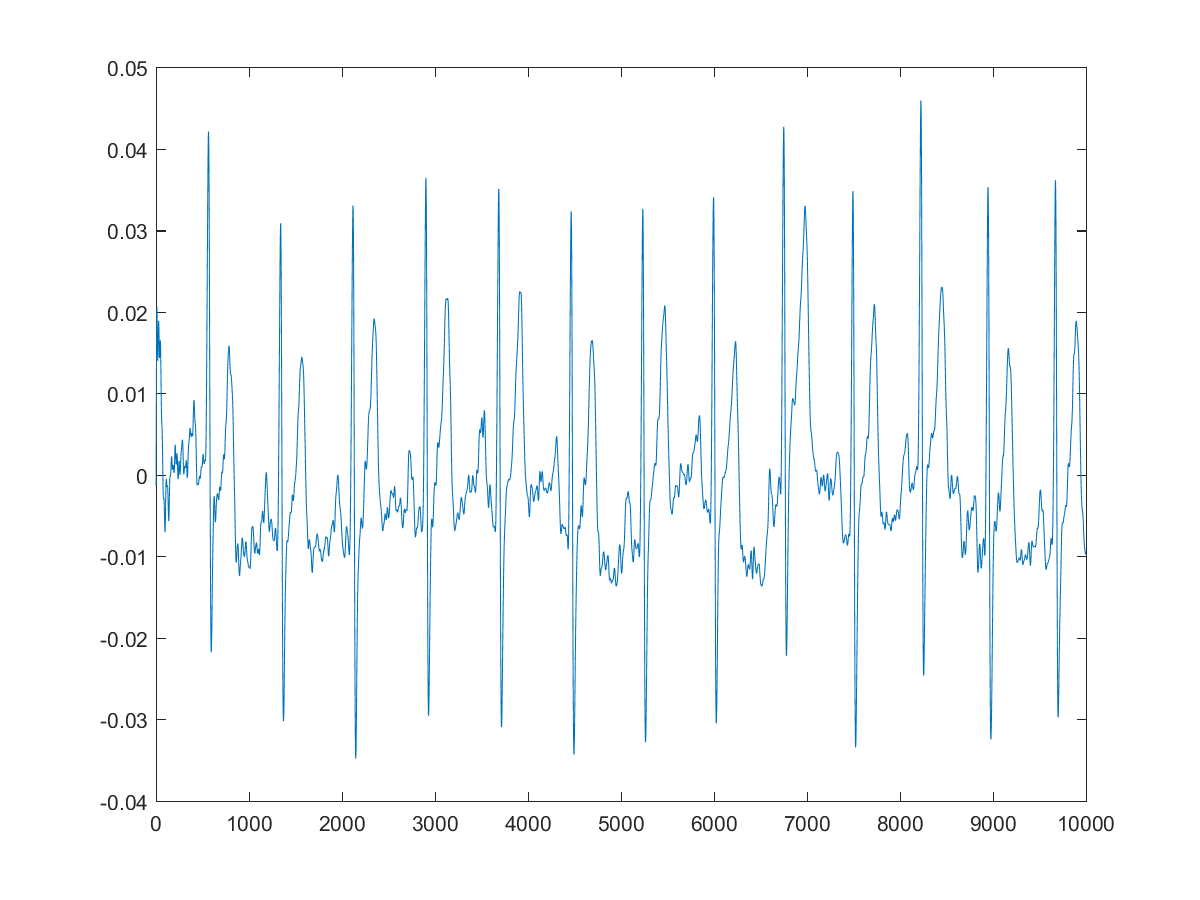
\includegraphics[width=1\linewidth]{filtered_ekg_hig}} \\b)
	\end{minipage}
	\vfill
	\begin{minipage}[h]{0.47\linewidth}
		\center{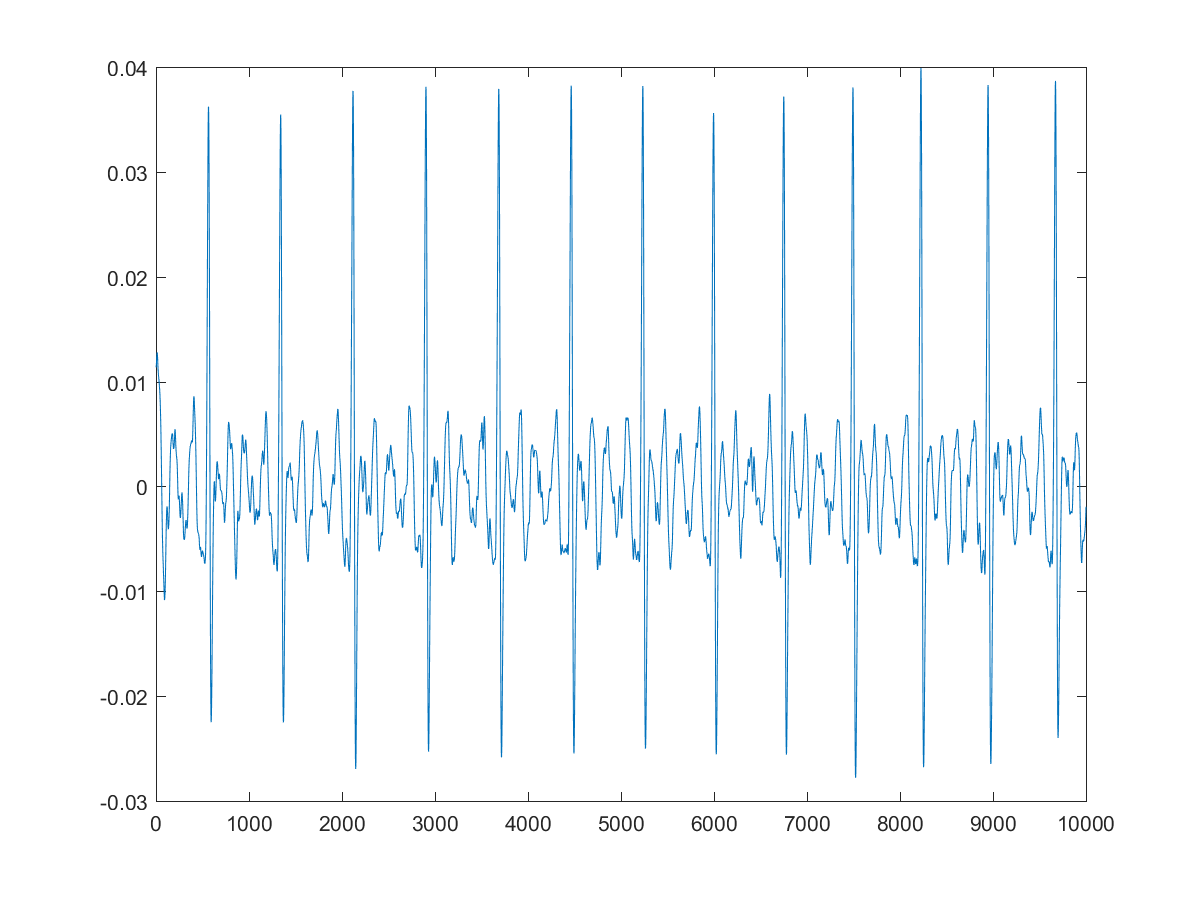
\includegraphics[width=1\linewidth]{filtered_ekg_low}} c) \\
	\end{minipage}
	\hfill
	\begin{minipage}[h]{0.47\linewidth}
		\center{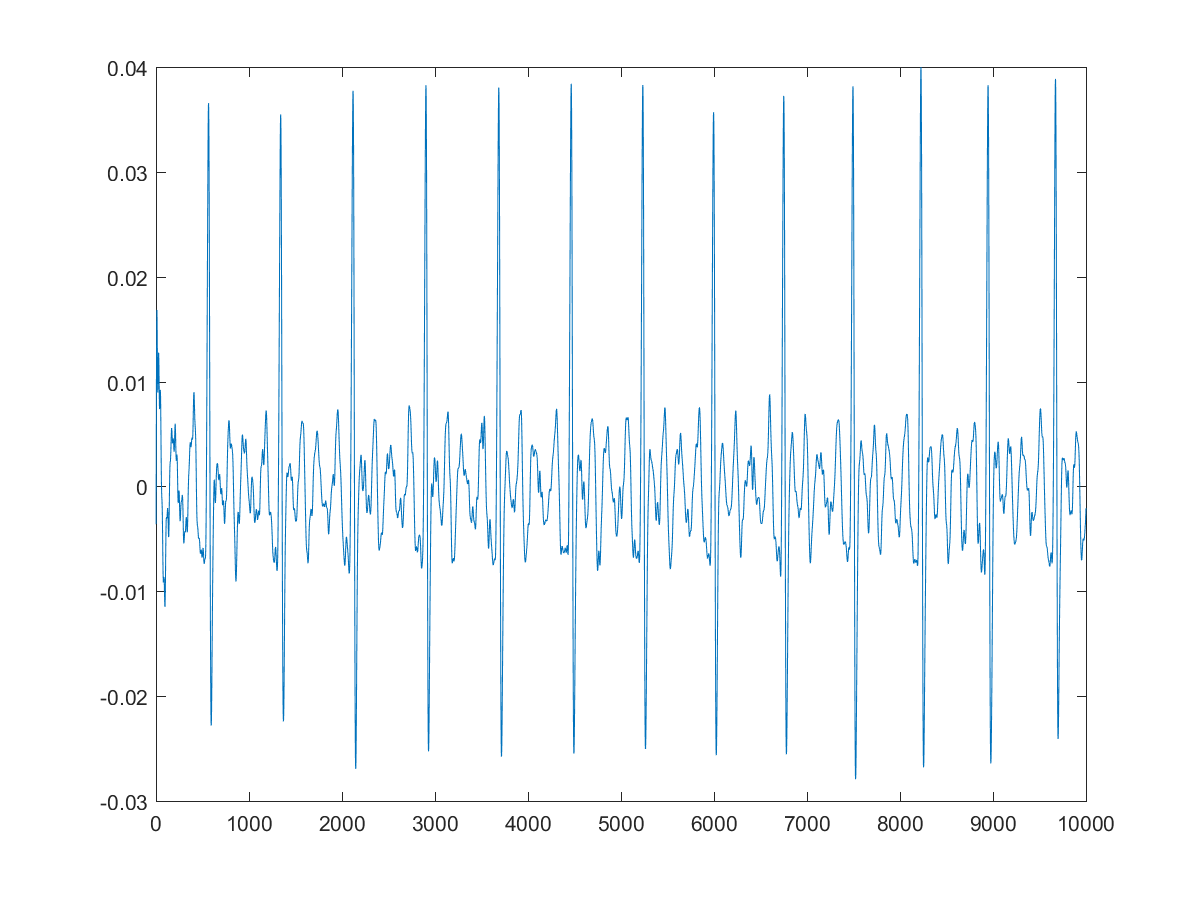
\includegraphics[width=1\linewidth]{filtered_ekg_low_hig}} d) \\
	\end{minipage}
	\caption{ЭКГ сигнал a)до фильтрации b) после высокочастотного фильтра
		c) после низкочастотного фильтра d) после обоих фильтров}
	\label{ris:filter_ekg}
\end{figure}

Для определения RR-пиков отбирались точки $i$ ЭКГ сигнала такие, что $x_i$ - локальный максимум в окне $[x_{i-k\_pred}, ..., x_i,    , x_{i+k\_next}]$, а также $min([x_{i-r\_pred}, ..., x_i])<0$ и $min([x_i, ..., x_{i+r\_next}])<0$. То есть сигнал справа и слева от локального минимума опускается ниже нуля. Напомню, что мы работаем с фильтрованным сигналом, среднее значение которого лежит около нуля.

Далее, когда мы определили координаты пиков на фильтрованном сигнале - находим обратным преобразванием их на исходном. Признаки, считаемые по QRS-комплексу считались по неотфильтрованныму сигналу, дабы не потерять информацию. Фильтр низких частот, применение которого желательно при поиске пиков, очень сильно искажает сигнал. 

\section{Работа с RR-сигналом}

Сигнал ЭКГ, собираемый носимыми устройствами, подвержен влиянию множества шумов. На него могут влиять следующие факторы, никак напрямую не связанные с сердцем.

\begin{itemize}
	\item Погрешности устройства
	\item Неплотное прилегание устройства к коже
	\item Подвижность человека
	\item Физические реакции, не связанные с сердечной деятельность (к примеру, внезапные сокращения мышц при засыпании, резкие движения, удары тока или другие различные причины)
\end{itemize}

Из-за этих причин при записи сигнала возникают лишние пики и теряются реально существующие (часть сигнала представляет собой константу). При первичной обработке RR-сигнала вырезались длительные участки сигнала без пиков (если на протяжени 2 минут не было пиков), и выкидывались участки сигнала между пиками, расположенными ближе чем 200 мс.


\section{Проведенные экперименты}

В рамках данного исследования решались следующие задачи.

\subsection{Предсказание сна}
Перед нами стояла задача по заданному RR-сигналу определить периоды сна и бодрствования для каждого человека. Данная задача представляет интерес, так как продолжительность сна является важным маркером здоровья. Также это может иметь дальнейшее применение в качестве будильников для дальнобойщиков и водителей, которые ездят ночью. Можно считывать сигнал с фитнес-браслета или холтера в реальном времени и, проанализировав его, посылать сигналы (вибрацию, звуковые), когда человек засыпает.

При анализе сигнал разбивался на временные промежутки определенной длительности. Для каждого полученного промежутка определялось состояние человека (спит или бодрствует). 

Необходимо помнить, что при решении данной задачи всегда будет присутствовать определенная погрешность. Процесс погружения в сон не моментален и обычно занимает некоторый промежуток времени.

Важно выбрать не слишком короткий и не слишком длинный промежуток времени для анализа. Если он будет коротким, на него будут сильно влиять различные мгновенные причины (такие как случайные движения, непроизвольные сокращения мышц и др., которые не были найдены и удалены во время фильтрации), не имеющие отношения к сердцебиению и состоянию организма. Он не должен быть слишком длинным - чем длиннее данный промежуток, тем больше погрешность определения границ сна. При анализе достаточно длительного промежутка могут быть потеряны различные высокочастотные особенности, которые будут усреднены. Оптимальным по длительности был признан промежуток в 5 минут.

В ходе данного исследования эта задача решалась следующими методами.
\subsubsection{Поиск максимально длинной подпоследовательности}

Если смотреть на RR-сигнал во время сна и бодрствования (рис. \ref{ris:rr_sleep_wake}), можно заметить, что во время сна частота пульса уменьшается (достаточно очевидное предположение, известное всем).

\begin{figure}[h]
	\begin{center}
		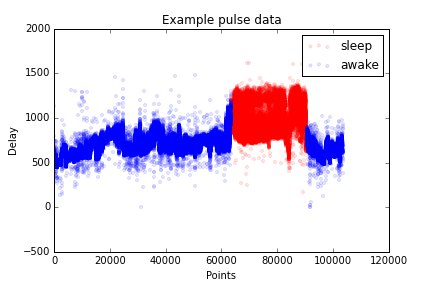
\includegraphics[scale=1]{wakesleeprr}
		\caption{Сигнал во время сна и бодрствования}
		\label{ris:rr_sleep_wake}
	\end{center}
\end{figure}

Первым предложенным алгоритмом был следующий.

Для каждых 200 отсчетов RR-сигнала ($\sim 5$ минут) подсчитывались средние значения. Далее анализируется последовательность средних, определяется граница с погрешностью в 100 отсчетов (половина временного интервала, по которому считались признаки).
\begin{enumerate}
	\item Подсчитываем среднее и дисперсию для анализируемой последовательности.
	\item Разбиваем все точки сигнала на три группы:
	\begin{itemize}
		\item точки больше среднего значения ($if\ mean_i > mean(all\ signal\ mean)$));
		\item точки на половину дисперсии меньше среднего значения ($if\ mean_i < mean(all\ signal\ mean) - 0.5std(all\ signal\ mean)$));
		\item все остальные точки.
	\end{itemize}
	\item Далее мы ищем наиболее длинную последовательность точек из первой группы, начинающуюся с 10 последовательных точек, не прерываемую более чем 5 точками из второй группы в любом ее месте. Помним, что в данном контексте точка -- это среднее двухсот отсчетов RR-сигнала.
\end{enumerate}

Средняя ошибка определения границ -- $\sim$ час.

Точность предсказания -- $\sim$ 70\%

На 80\% тестовой выборки абсолютная ошибка составила менее 30 минут.
\begin{figure}[h]
	\begin{minipage}[h]{0.47\linewidth}
		\center{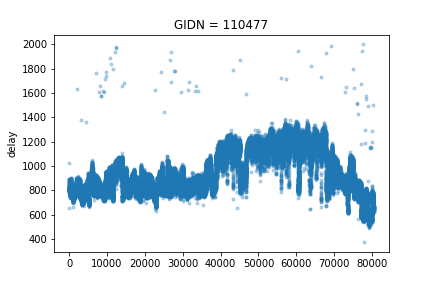
\includegraphics[width=1\linewidth]{1104770}} a) \\
	\end{minipage}
	\hfill
	\begin{minipage}[h]{0.47\linewidth}
		\center{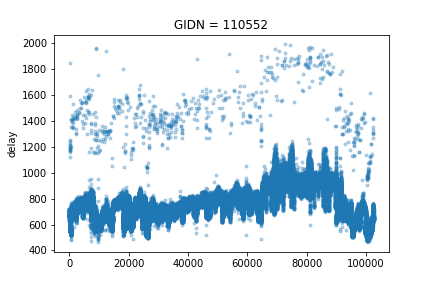
\includegraphics[width=1\linewidth]{1105520}} \\b)
	\end{minipage}
	\vfill
	\begin{minipage}[h]{0.47\linewidth}
		\center{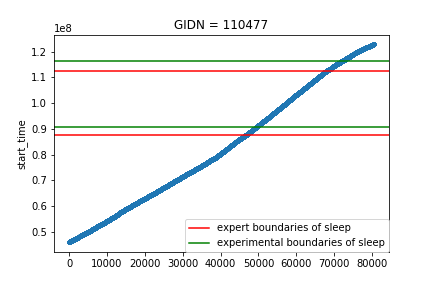
\includegraphics[width=1\linewidth]{1104771}} c) \\
	\end{minipage}
	\hfill
	\begin{minipage}[h]{0.47\linewidth}
		\center{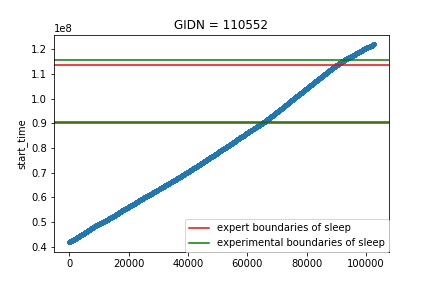
\includegraphics[width=1\linewidth]{1105521}} d) \\
	\end{minipage}
	\caption{RR-сигнал и границы найденного сна для двух людей}
	\label{ris:find_sleep_bound1}
\end{figure}
\subsubsection{Градиентный бустинг над деревьями}

Было принято решение увеличить количество признаков и кроме среднего посчитать характеристики, которые считаются информативными для работы с RR-сигналом. Для предсказания сна RR сигнал разбивался на участки по 200 отсчетов ($\sim$ 5 минут). Для каждого участка подсчитывались признаки, которые потом подавались на вход алгоритму классификации.
Считали следующие признаки:

\begin{itemize}
	\item mean -- среднее по всему сигналу
	\item std -- дисперсия всего сигнала
	\item EBS -- разница между максимальным и минимальным значения RR-сигнала
	
	Перечисленные выше признаки считались для всего сигнала. Далее идут признаки подсчитанные для каждых 200 отсчетов.
	
	\item mean window -- среднее значений на 200 отсчетах
	\item std window -- дисперсия на 200 отсчетах
	\item EBS window -- значение EBS, посчитанное по каждым 200 отсчетам
	\item NN50 -- количество двух последовательных RR-интервалов, отличающихся на 50 миллисекунд
	\item pNN50 -- NN50 / 200
	\item NN20 -- количество двух последовательных RR-интервалов, отличающихся на 20 миллисекунд
	\item pNN20 -- NN20 / 200
	\item entropy -- энтропия сигнала
	\item spectr entropy -- спектральная энтропия
\end{itemize}

Вектор признаков, подсчитанный для каждого пятиминутного интервала, подавался на вход классификатору. Были проведены эксперименты со случайными лесами, логистической регрессией, методом к-ближайщих.

С помощью кросс-валидации были подсчитаны ошибки для наиболее оптимальных при этой задаче параметров алгоритмов.
Наилучшее качество показал бустинг над случайными лесами:

\begin{tabular}{|c|c|c|}
	\hline \rule[-2ex]{0pt}{5.5ex} true/pred & awake & sleep \\ 
	\hline \rule[-2ex]{0pt}{5.5ex} awake & 0,85 & 0,15 \\ 
	\hline \rule[-2ex]{0pt}{5.5ex} sleep & 0,29 & 0,71 \\ 
	\hline 
	
\end{tabular}\\

Точность предсказания составила 80\%.

\subsubsection{Предсказание сна с помощью нейросетевых методов}

Было предположено, что для адекватной работы архитектуры хватит всего 4 простых признаков: среднего и дисперсии для каждого временного отрезка, среднего и дисперсии сигнала для всего сигнала человека.

Погружение в сон -- это не мгновенный процесс, поэтому необходимо каким-либо образом сохранять информацию о текущем состоянии человека и передавать ее дальше. Для решения этой задачи были использованы рекуррентные нейронные сети с LSTM нейронами. 

Особенностью архитектуры LSTM нейрона является наличие гейта памяти, с которым можно проделывать следующие операции:

\begin{itemize}
	\item записать информацию в гейт;
	\item обнулить внутреннее состояние гейта;
	\item получить информацию из гейта.
\end{itemize}

Была реализована следующая архитектура сети. рис \ref{ris:arh_rnn}

\begin{figure}[h]
	\begin{center}
		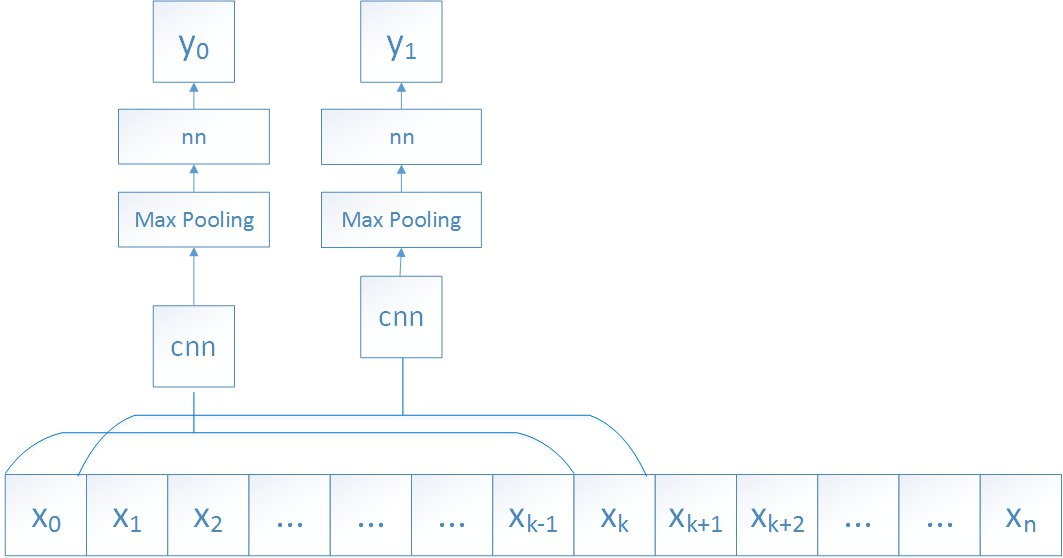
\includegraphics[scale=0.36]{arch_rnn}
		\caption{Реализованная архитектура сети}
		\label{ris:arh_rnn}
	\end{center}
\end{figure}

Для каждого 5-ти минутного интервала подсчитывались признаки $X_i$ (средние и дисперсии). Далее вектор подсчитанных признаков подавался на вход рекуррентному слою со 100 нейронами. Далее шел полносвязный слой, выход которого уже шел на заключительный нейрон, который и выдавал информацию о состоянии человека во время этого интервала. Регуляризация и слои с dropoutом не использовались. После каждой эпохи обучения считалось качество на валидационной выборке, и сохранялись только модели, которые уменьшали на ней ошибку (а не только на обучающей выборке). 

Были случайным образом отобраны 1200 человек для обучения, 300 для тестирования и 300 для валидации. 
Чтобы убедиться, что результат не зависит от отбора людей в обучающую и валидационную выборки, эксперимент был проведен несколько раз с различными разбиениями.

Полученная точность (при tnr == tpr) -- 85\%. 

Несмотря на простоту признаков, этот метод дал лучшее качество классификации, чем предложенные ранее. К тому же его можно настроить (меняя пороговое значение), чтобы он мог предсказывать момент наступления сна чуть ранее, чем когда он наступит в действительности -- это достаточно актуально для применения в качестве будильника для водителей.

Были реализованы различные вариации данной архитектуры. Менялось количество нейронов в LSTM слое, убирался полносвязный слой после. Влияние количества нейронов можно увидеть на рис. \ref{ris:roc_rnn}.

\begin{figure}[h!]
	\begin{center}
		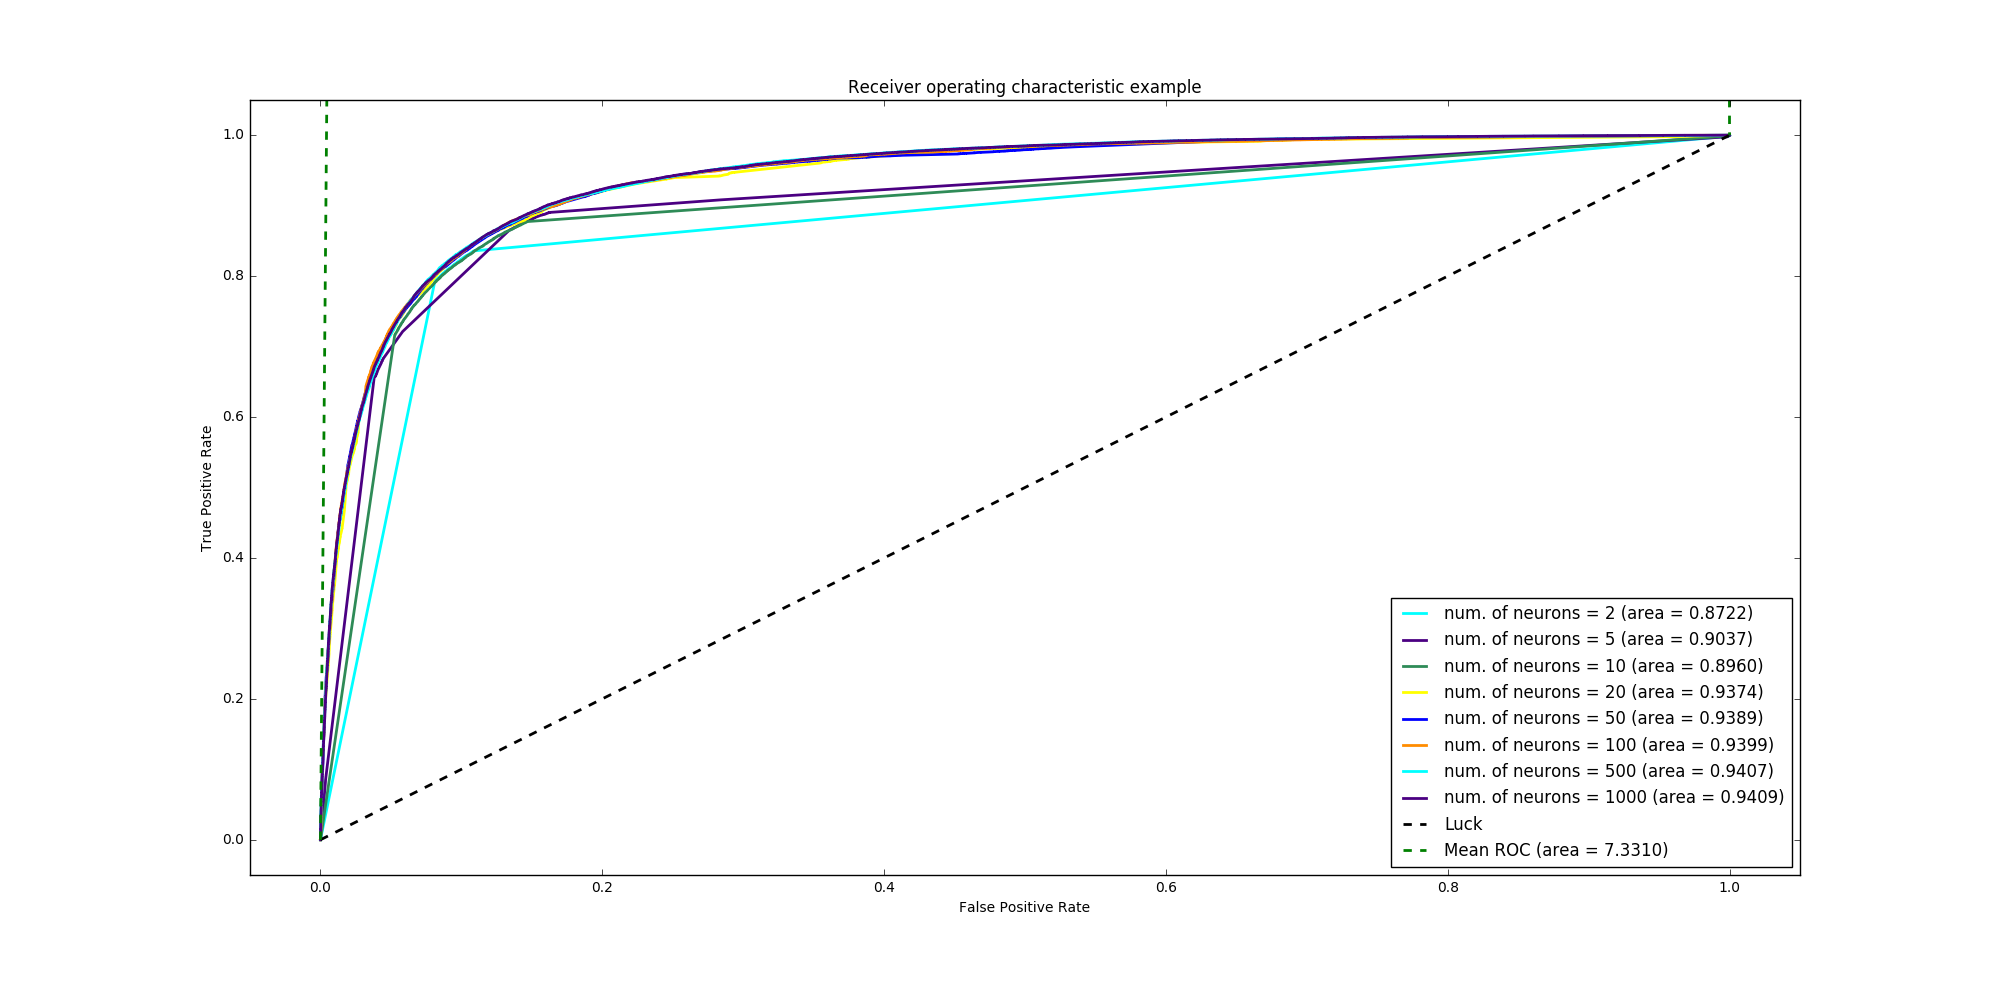
\includegraphics[scale=0.36]{ROC_curve_for_dif_hidden_neuron}
		\caption{ROC кривые для различного количество нейронов в рекуррентном слое}
		\label{ris:roc_rnn}
	\end{center}
\end{figure}

После сети размеченный сигнал обрабатывался морфологическими фильтрами "открытие", "закрытие". Это делалось для фильтрации одиночных выбросов. К примеру когда есть последовательность временных интервалов, размеченных как сон, и среди них один или несколько помечены как состояние бодрствования. Данные фильтры помечают эти интервалы как сон. Также возможна обратная ситуация.

\subsubsection{Эксперименты со сверточными сетями}

Также в процессе работы было проведено следующее исследование. Был интересен следующий вопрос: можно ли добиться подобного качества или улучшить его, используя сверточную сеть, считывающую несколько векторов признаков. По аналогии с предыдущей архитектурой была реализована следующая модель (рис. \ref{ris:arh_cnn}).  

\begin{figure}[h!]
	\begin{center}
		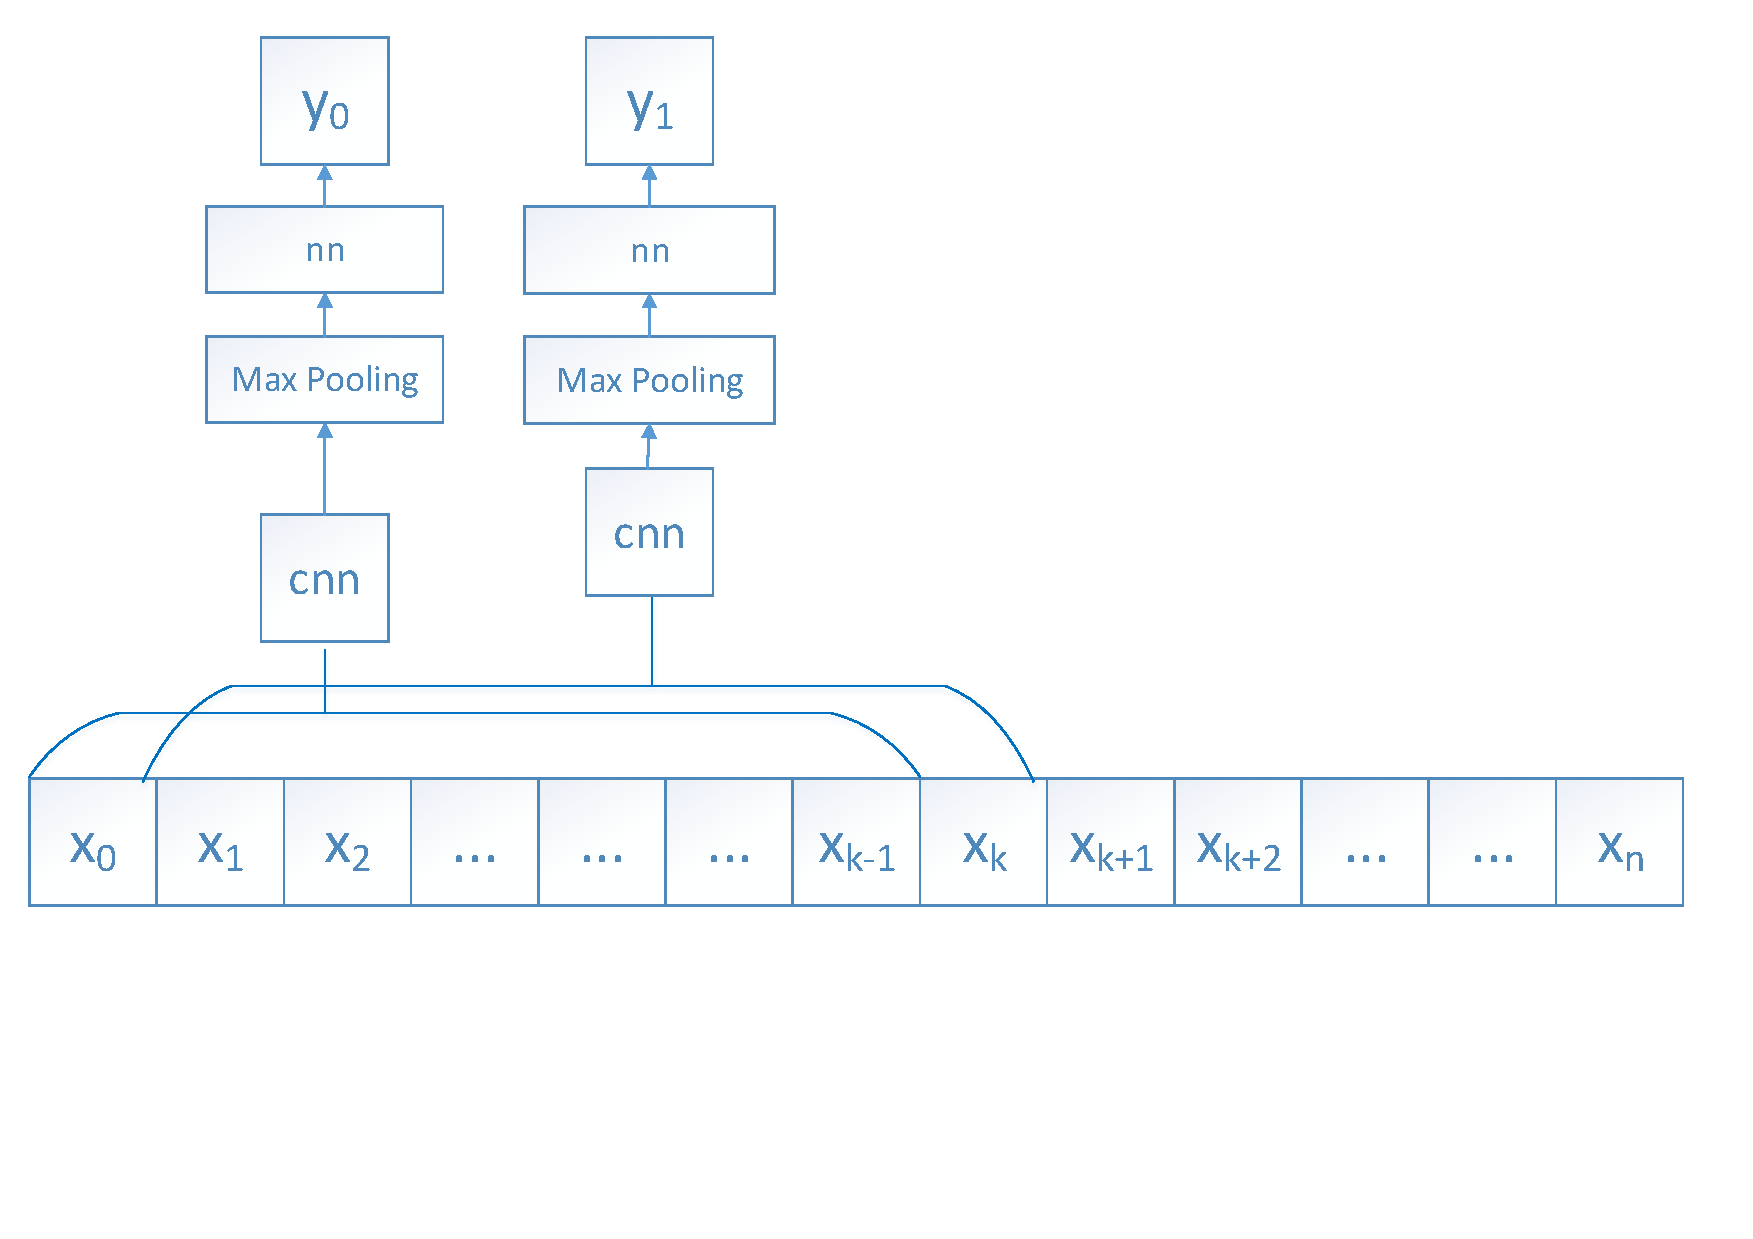
\includegraphics[scale=0.36]{arch_cnn}
		\caption{Реализованная архитектура сверточной сети}
		\label{ris:arh_cnn}
	\end{center}
\end{figure}

Для каждого 5-ти минутного интервала подсчитывались признаки $X_i$ (средние и дисперсии). Далее $k$ векторов подсчитанных признаков подавались на вход сверточному слою. Далее шли слой пулинг и полносвязный, выход которого уже шел на заключительный нейрона. Выход заключительного нейрона предсказывал состояние человека, соответствующее времени $k/2$ вектора из поданных. Были проведены эксперименты с разным количеством фильтров и их шириной в сверточном слое. Лучшее качество показали фильтры длины 3.

Для различного количества $k$ признаков были проведены эксперименты. Результаты можно наблюдать на рис. \ref{ris:roc_cnn}.

\begin{figure}[h!]
	\begin{center}
		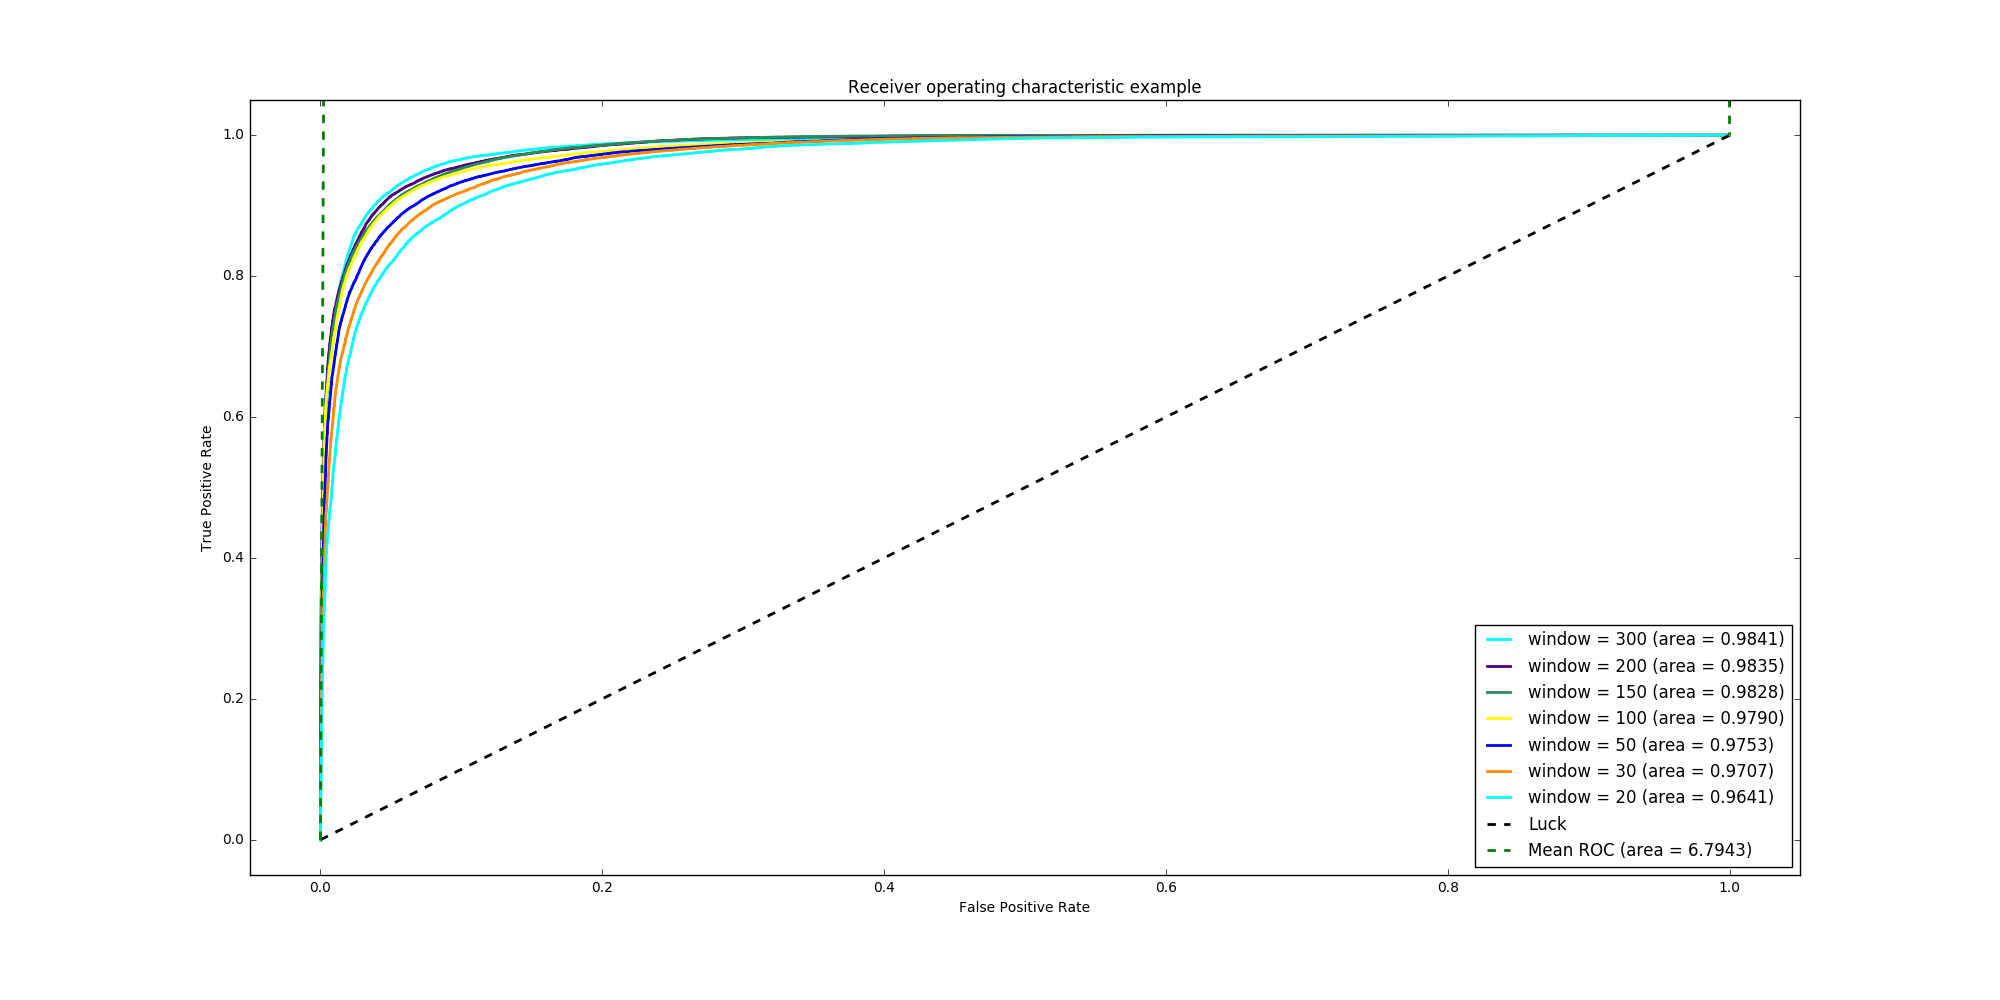
\includegraphics[scale=0.36]{ROC_cnn_filteres_len_3_21d_curve_for_dif_step}
		\caption{ROC кривые для различных входных данных сверточного слоя различной ширины}
		\label{ris:roc_cnn}
	\end{center}
\end{figure}

Для $k = 5 $  ($\sim 25$ минут) векторов входного слоя качество (при tnr == tpr) - 81\%.

Для $k = 50$ ($\sim 4$ часа) векторов входного слоя качество (при tnr == tpr) - 90\%.

Если на вход сети давать достаточно большой временной отрезок, сверточная сеть превосходит качеством рекуррентную. При чем, как показали эксперименты, не обязательно обучать сверточную сеть. На таком объеме входных данных можно обучить простую двухслойную полносвязную сеть со схожим качеством предсказания. Однако данный метод не применим в системах, работающих в реальном времени, так как для задачи предсказания момента погружения в сон, опоздание на 15 минут будет существенным. Поэтому лучшие архитектурой для предсказания сна по RR-сигналу в режиме реального времени была признана рекуррентная сеть.
 
Однако, если сигнал уже собран и его необходимо только разметить -- а такие задачи ставятся в медицине -- данная архитектура является более подходящей, так здесь важнее качество разметки.

\subsection{Предсказания пола и возраста}

Определение заболеваний по ЭКГ достаточно сложная задача. К началу ее исследования хотелось бы иметь набор характеристик, про которые точно можно сказать, что они информативны и содержат информацию о человеке.
Для этого было решено реализовать предсказание пола и возраста человека, так как это более простая задача, и исследовать информативность признаков.

Анализ информативности признаков проводился следующим образом.
\begin{itemize}
	\item на вход классификатору подалась часть признаков и оценивалась точность классификации.
	\item далее было выбрано наименьшее подмножество признаков.
\end{itemize}	

Было увеличено количество признаков, и кроме временных характеристик сигнала считались характеристики, которые упоминаются в других исследованиях.

Считались следующие информативные признаки:
\begin{itemize}
	\item mean -- среднее по всему сигналу
	\item std mean -- отклонение последовательности средних значений на 200 отсчетах RR сигнала от среднего по всему сигналу
	\item mean std -- среднее значений дисперсии на 200 отсчетах
	\item std std -- дисперсия дисперсий, посчитанных по 200 отсчетам RR-сигнала
	\item EBS -- разница между максимальным и минимальным значения RR-сигнала
	\item mean EBS -- среднее значение EBS, посчитанное по каждым 200 отсчетам
	\item std EBS
	\item NN50 -- количество двух последовательных RR-интервалов, отличающихся на 50 миллисекунд
	\item pNN50 -- NN50 / len(RR-сигнала)
	\item NN20 количество двух последовательных RR-интервалов, отличающихся на 20 миллисекунд
	\item pNN20 -- NN20 / len(RR-сигнала)
	
    Изначально признаки подсчитывались отдельно для всего сигнала, для сигнала во время сна, для сигнала во время периода бодрствования. Но было показано, что достаточно подсчитывать признаки только для исходного сигнала. Качество при этом падало незначительно. 

	\item down percentile -- 5\% квантиль справа
	\item up percentile -- 5\% квантиль слева
	\item entropy -- энтропия сигнала
	\item spectr entropy -- спектральная энтропия
	
	Предполагается, что значение RR-интервалов отличаются в периоды сна и бодрствования, и что их можно разделить на 2 кластера. RR-сигнал представлялся в виде смеси двух гаусовских распределений. Следующие признаки - характеристики этой смеси. 
	
	\item gmm mean1 -- математическое ожидание первого распределения
	\item gmm mean2 -- математическое ожидание второго распределения
	\item gmm weight1 -- процент элементов сигнала, отнесенных к первому распределению.
	\item gmm std1 -- дисперсия первого распределения
	\item gmm std2 -- дисперсия второго распределения
	
	Эти признаки оказались неинформативными.
	
	Также подсчитывались геометрические характеристики сигнала
	
	\item fractal dim -- фрактальная размерность
	\item hjorth dim, hjorth mobility, hjorth complexity -- спектральные параметры сигнала : размерность, мощьность, изменчивость
	\item kurtosis -- четвертый момент сигнала
	\item skewness -- третий момент сигнала
	\item spearmen cor 10, spearmen cor pvalue 10, spearmen cor 50, spearmen cor pvalue 50	
	,spearmen cor 100, spearmen cor pvalue 100, spearmen cor 500, spearmen cor pvalue 500 -- 
	параметры корреляции Спирмена с соответствующими параметрами
	%	\item angle cross - угол, под которым сходятся наглоны при подсчете значений автокореляции
\end{itemize}

Эти признаки подавались на вход градиентному бустингу над деревьями. 

Точность классификации пола человека -- 70\%.

Точность классификации возраста человека (все возможные значение возраста разбивались на 4 группы) -- 65\%


\subsection{Определение болезней}

Для определения заболеваний на вход алгоритму классификации подавались описанные в предыдущем разделе признаки. Данные эксперименты не увенчались успехом -- точность классификации колебалась в районе 50--55\% для различных болезней.

Для улучшения качества были предложены следующие подходы.

\subsubsection{Нарезка выборки}
Для классификации промежутков времени на сон/бодрствование необходим весь временной ряд. После фильтрации и выброса неподходящих интервалов его длительность составляла порядка 23 часов. Но для предсказания каких-либо характеристик человека достаточно только его части. Если брать в качестве входных данных признаки, посчитанные по небольшому участку сигнала, размер обучающей выборки увеличится в несколько раз. Вместе с этим должна увеличиться ее обобщающая способность.

То, что мы берем только участки сигнала позволяет нам отобрать участки с минимумом шума.
В данном исследовании нарезались отрезки длительностью 10 минут.

Было решено отбирать участки сигнала, где все выделенные R-пики удовлетворяют следующим условиям:

\begin{itemize}
	\item разница высот соседних пиков менее 20\%
	\item разница продолжительностей соседних RR интервалов менее 20\%
\end{itemize}

В большинстве случаев такие пики возникают как проявление нерегулярного ритма. Это проявление электрических импульсов, генерируемых не SA узлом, а случайными клетками соединительной ткани сердца. 

Также это более качественно отфильтровывало участки с сильной зашумленностью из-за физической активности человека. Недостатком этого отбора оказался следующий факт -- большая часть участков приходилась на время сна. Это логичное следствие, во время сна человек большую часть времени не двигается. После подобной нарезки выборка увеличилась $\sim$ в 20 раз.

\subsubsection{Подсчет дополнительных признаков}

Были добавлены частотные признаки, подсчитанные по фурье преобразованию сигнала, и признаки, подсчитанные по по QRS-комплексу. Для разметки QRS-комплекса использовались готовые алгоритмы из библиотеки ecgpuwave для среды разработки MATLAB.

\begin{figure}[h!]
	\begin{center}
		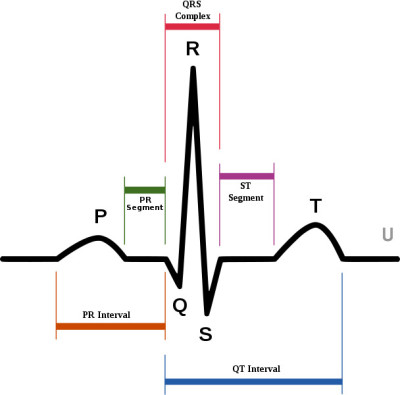
\includegraphics[scale=0.7]{QRS_for_features}
		\caption{QRS-комплекс}
		\label{ris:QRS}
	\end{center}
\end{figure}

Считались:

\begin{itemize}
	\item амплитуды QR, RS (разница между максимальными и минимальными значениями справа и слева от пика в некоторой окрестности);
	\item высота пика R по отношению к среднему уровню сигнала;
	\item разница высот между пиками P, R, T;
	\item отношения высот P, R, T;
	\item средние значения на промежутках PQ, QR, QT;
	\item длительность различных фаз в QRS-комплексе;
	\item площадь под графиком на промежутках PQ, QS, ST, begin-Q, S-final.
\end{itemize}


В медицине утверждается \cite{p_wave, T_wave}, что врачи ориентируются на данные параметры при постановки диагноза.
Для каждого вырезанного участка подсчитывались усредненные характеристики описанных выше величин.

\subsubsection{Предсказание болезней с помощью нейросетевых методов}

Далее обучалась двухслойная полносвязная сеть, на вход которой подавались признаки, подсчитанные по вырезанному участку сигнала. В качестве $y$ подавалась информация -- болеет человек данной болезнью или нет. Данные методы позволили немного улучшить качество предсказания, однако результаты получились далеко не обнадеживающими (53--65\% для различных болезней).

Такое низкое качество предсказание может быть объяснено следующими соображениями.
\begin{enumerate}
	\item У нас очень разнообразная выборка пожилых людей, все люди болеют сразу многими болезнями. Людей, у которых не найдено болезней всего 7 из 1800.
	\item Врачи, при постановке диагноза по ЭКГ сигналу обладают дополнительной информацией о человеке -- могут спросить его о курении, видят цвет лица, возраст, конституцию тела человека и многое другое. Так у здорового курящего человека и больного некурящего ЭКГ сигнал может быть очень похожим. У нас были только данные ЭКГ.
	\item  В медицине работают минимум с тремя отведениями (обычно с двенадцатью). У нас было только одно.
\end{enumerate}

\subsubsection{Предсказание болезней с помощью кодограмм}

Также был повторен метод К.В.Воронцова, описанный ранее. Его результаты впечатляли, и хотелось добиться похожих. Он был реализован согласно описанию из статьи. Однако качество предсказаний не улучшилось. 

\begin{figure}[h!]
	\begin{center}
		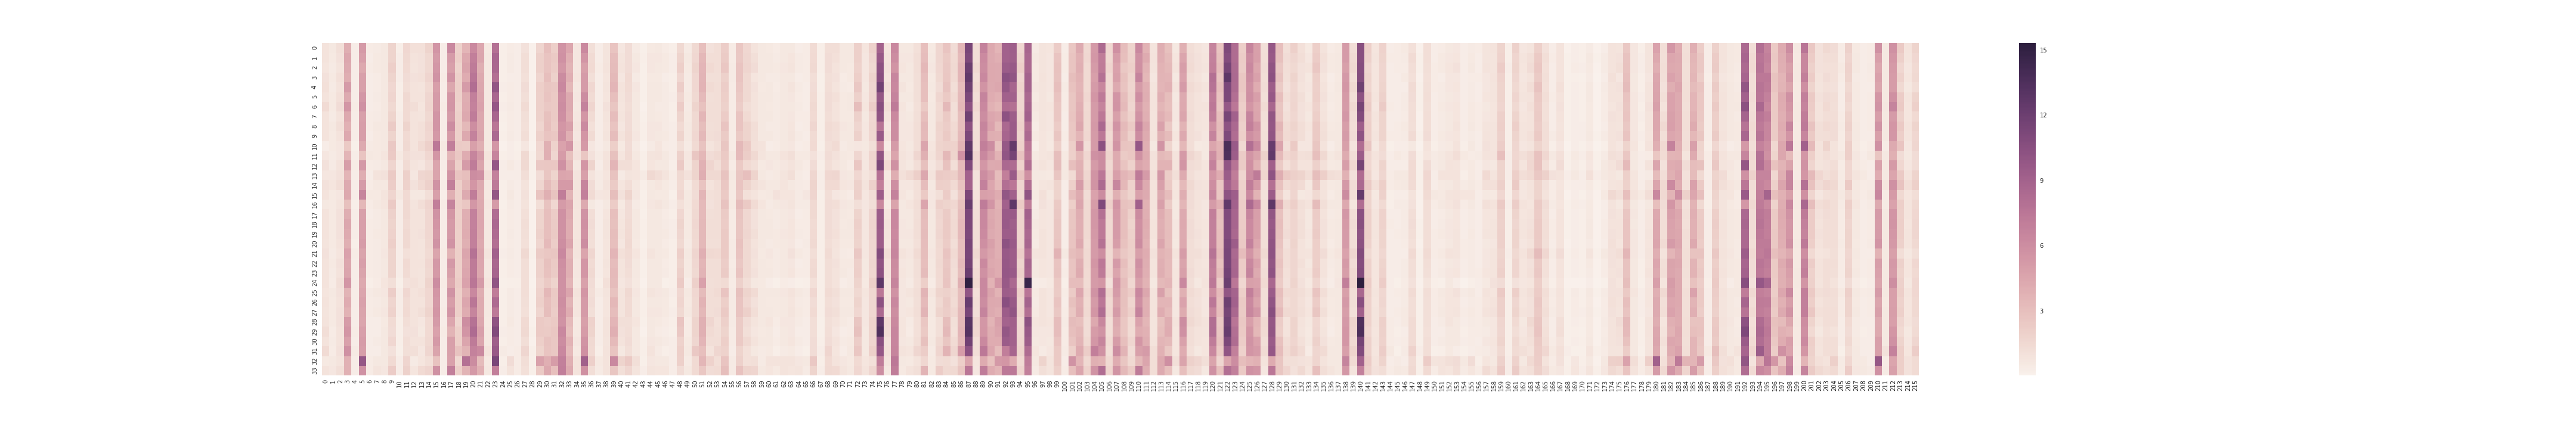
\includegraphics[scale=0.14]{hist_trigramm_to_illness_first_all}
		\caption{Частоты триграмм для различных болезней. По оси $x$ - номер триграммы, по оси $y$ - номер болезни}
		\label{ris:trigramm}
	\end{center}
\end{figure}

Информативными оказались триграммы только для очень сильно несбалансированных классов болезней $(1:100)$, таких как эпилепсия (больных - 14), рак кожи (больных - 21), болезнь паркинсона (больных - 29). Скорее всего эти триграммы информативны, так предсказывают конкретных людей, а не болезнь.

Также наша задача, в отличии от решаемой Воронцовым, усложнялась следующими фактами.
\begin{itemize}
	\item Воронцов отделял класс абсолютно здоровых людей (курсанты военных училищ) от эталонной (подготовленной врачами для каждой болезни отдельно) выборки больных. "По каждому заболеванию $y_m$ была отобрана выборка $X_m$, состоящая только из тех случаев, в которых наличие специфического патоморфологического субстрата данного заболевания было надёжно установлено. Особенно тщательно была сформирована выборка $X_0$ здоровых людей разного пола и возраста, не имеющих существенных отклонений от состояния нормы. В экспериментах выборки больных $X_m$ по каждому заболеванию $y_m$ сравнивались с одной и той же выборкой здоровых $X_0$."
	
	У нас имелось всего 7 абсолютно здоровых пожилых людей, и мы не могли точно воспроизвести данный эксперимент. Мы отделяли людей больных конкретной болезнью, от не больных именно ей (но возможно, даже скорее всего, больных какой-либо другой болезнью)
	\item Также сигнал ЭКГ, анализируемый в его работах, снимался в течение 15 минут, когда человек спокойно сидел на стуле, а устройство точно было хорошо к нему подсоединено. Это позволило им сразу избавиться от большинства шумов, появляющихся при получении данных с холтеровских мониторов. 
\end{itemize}

Из-за этих причин не удалось успешно применить подход, описанный в работах Воронцова к нашим данным. Качество классификации оставалось на уровне 55\% - 60\%. Такое качество вполне может быть достигнуто случайным классификатором.


